\documentclass[tikz,border=3mm]{standalone}
\usepackage[T1]{fontenc}
\usepackage{helvet}
\renewcommand{\familydefault}{\sfdefault}
\usepackage{amsmath,amssymb}
\usepackage{tikz}
\usetikzlibrary{shapes.geometric, positioning, arrows.meta, calc}

\begin{document}
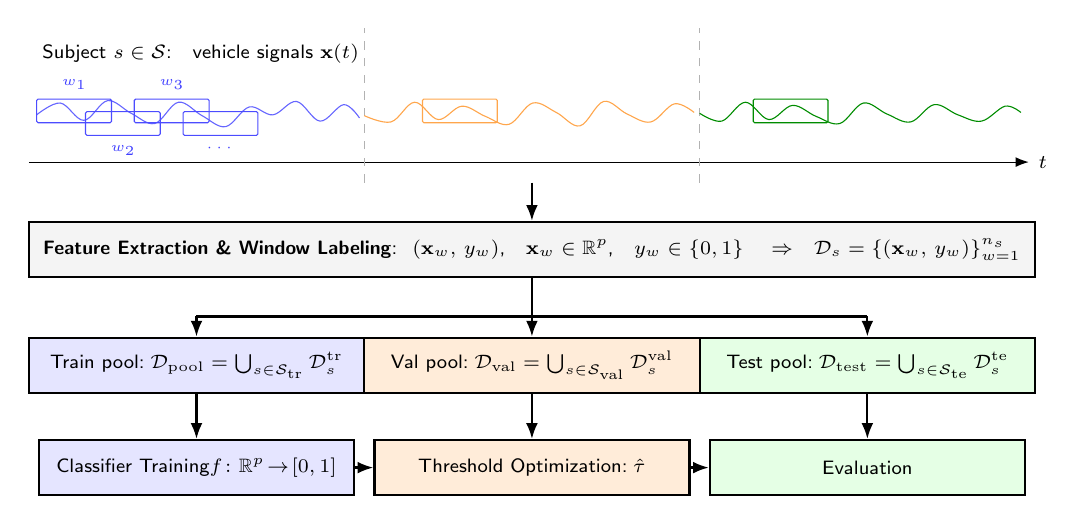
\begin{tikzpicture}[
  every node/.style={font=\sffamily\scriptsize},
  >=Latex,
  %% Uniform box style: thick border, white fill
  pbox/.style={draw=black, thick, rectangle, fill=white, align=center,
               minimum height=7mm, inner xsep=5pt, inner ysep=3pt},
  %% All arrows identical
  arr/.style={-{Latex[length=2.0mm, width=1.5mm]}, thick},
]

%% ============================================================
%% Layout (all units cm, figure width W=12.78):
%%   Equal-thirds:
%%     Train:  x = 0    .. 4.26  (cx = 2.13)
%%     Val:    x = 4.26 .. 8.52  (cx = 6.39)
%%     Test:   x = 8.52 .. 12.78 (cx = 10.65)
%%   Signal strip: y = -0.68 .. 1.28  (south=-0.68)
%%   Feat box:     center y = -1.53   (south ≈ -1.88)
%%   gap = 0.50cm everywhere
%%   Bus (T-junction): y = -2.38
%%   Pool row:     center y = -3.00   (top ≈ -2.60)
%%   Pipeline row: center y = -4.30
%% ============================================================

%% ==================================================================
%% SECTION A: Time-series signal strip
%% ==================================================================


%% Label above all window frames
\node[anchor=west, font=\sffamily\scriptsize] at (0.05, 0.96)
  {Subject $s \in \mathcal{S}$:\quad vehicle signals $\mathbf{x}(t)$};

\draw[->, thin] (0,-0.42) -- (12.7,-0.42) node[right]{$t$};

%% Dashed separators at equal-third boundaries
\draw[dashed, gray!60, thin] (4.26,-0.68) -- (4.26,1.28);
\draw[dashed, gray!60, thin] (8.52,-0.68) -- (8.52,1.28);

%% Signal traces shifted up +0.16 from waveform zone (y in [-0.12, 0.38])
\draw[thin, blue!60, smooth, tension=0.6] plot coordinates {
  (0.1,0.18)(0.4,0.33)(0.7,0.11)(1.0,0.36)(1.3,0.20)
  (1.6,0.07)(1.9,0.34)(2.2,0.17)(2.5,0.03)(2.8,0.28)
  (3.1,0.18)(3.4,0.35)(3.7,0.10)(4.0,0.31)(4.2,0.14)};
\draw[thin, orange!70, smooth, tension=0.6] plot coordinates {
  (4.26,0.17)(4.6,0.09)(4.9,0.34)(5.2,0.12)(5.5,0.29)
  (5.8,0.16)(6.1,0.06)(6.4,0.33)(6.7,0.21)(7.0,0.04)
  (7.3,0.35)(7.6,0.19)(7.9,0.09)(8.2,0.32)(8.45,0.21)};
\draw[thin, green!55!black, smooth, tension=0.6] plot coordinates {
  (8.52,0.20)(8.8,0.10)(9.1,0.34)(9.4,0.12)(9.7,0.30)
  (10.0,0.16)(10.3,0.07)(10.6,0.33)(10.9,0.19)(11.2,0.09)
  (11.5,0.31)(11.8,0.18)(12.1,0.10)(12.4,0.29)(12.6,0.21)};

%% Sliding windows: staggered vertically (stride < width → overlap)
%%   Width = 0.95cm, stride = 0.62cm
%%   Upper row: y = 0.08 .. 0.38;  Lower row: y = -0.08 .. 0.22
\draw[blue!70, thin, rounded corners=0.5pt]  (0.10,0.08) rectangle (1.05,0.38); % w1 up
\draw[blue!70, thin, rounded corners=0.5pt]  (0.72,-0.08) rectangle (1.67,0.22); % w2 lo
\draw[blue!70, thin, rounded corners=0.5pt]  (1.34,0.08) rectangle (2.29,0.38); % w3 up
\draw[blue!70, thin, rounded corners=0.5pt]  (1.96,-0.08) rectangle (2.91,0.22); % w4 lo
\node[font=\sffamily\tiny, text=blue!75, anchor=south] at (0.58, 0.38)  {$w_1$};
\node[font=\sffamily\tiny, text=blue!75, anchor=north] at (1.20,-0.08)  {$w_2$};
\node[font=\sffamily\tiny, text=blue!75, anchor=south] at (1.82, 0.38)  {$w_3$};
\node[font=\sffamily\tiny, text=blue!75, anchor=north] at (2.44,-0.08)  {$\cdots$};

\draw[orange!70, thin, rounded corners=0.5pt] (5.00,0.08) rectangle (5.95,0.38);
\draw[green!55!black, thin, rounded corners=0.5pt] (9.20,0.08) rectangle (10.15,0.38);

%% ==================================================================
%% SECTION B: Feature Extraction box (cx = 6.39)
%% ==================================================================
\node[pbox, fill=gray!9, minimum width=12.78cm] (feat) at (6.39,-1.53)
  {\textbf{Feature Extraction \& Window Labeling}:\;
   $(\mathbf{x}_w,\,y_w)$,\quad $\mathbf{x}_w \in \mathbb{R}^p$,\quad $y_w \in \{0,1\}$
   \quad$\Rightarrow$\quad
   $\mathcal{D}_s = \{(\mathbf{x}_w,\,y_w)\}_{w=1}^{n_s}$};

%% ==================================================================
%% SECTION C: Split & Pool nodes (partition bar removed; merged into one row)
%%   T-junction bus at y = -2.38 distributes feat output to 3 boxes
%%   Box centers at y = -3.00
%% ==================================================================

%% Train column (cx = 2.13)
\node[pbox, fill=blue!10, minimum width=4.26cm] (pool) at (2.13,-3.00)
  {Train pool:\;$\mathcal{D}_{\mathrm{pool}}
    = \bigcup_{s \in \mathcal{S}_{\mathrm{tr}}} \mathcal{D}_s^{\mathrm{tr}}$};

%% Val column (cx = 6.39)
\node[pbox, fill=orange!15, minimum width=4.26cm] (valp) at (6.39,-3.00)
  {Val pool:\;$\mathcal{D}_{\mathrm{val}}
    = \bigcup_{s \in \mathcal{S}_{\mathrm{val}}} \mathcal{D}_s^{\mathrm{val}}$};

%% Test column (cx = 10.65)
\node[pbox, fill=green!10, minimum width=4.26cm] (testp) at (10.65,-3.00)
  {Test pool:\;$\mathcal{D}_{\mathrm{test}}
    = \bigcup_{s \in \mathcal{S}_{\mathrm{te}}} \mathcal{D}_s^{\mathrm{te}}$};

%% ==================================================================
%% SECTION D: Pipeline nodes — center y = -4.30
%% ==================================================================

%% Train column (cx = 2.13)
\node[pbox, fill=blue!10, minimum width=4.0cm] (cls) at (2.13,-4.30)
  {Classifier Training\newline
   $f\colon\mathbb{R}^p\!\to\![0,1]$};

%% Val column (cx = 6.39)
\node[pbox, fill=orange!15, minimum width=4.0cm] (thr) at (6.39,-4.30)
  {Threshold Optimization:\;$\hat{\tau}$};

%% Test column (cx = 10.65)
\node[pbox, fill=green!10, minimum width=4.0cm] (evl) at (10.65,-4.30)
  {Evaluation};

%% ==================================================================
%% All arrows
%% ==================================================================

%% Signal strip → feat
\draw[arr] (6.39,-0.68) -- (feat.north);

%% feat → T-junction bus → 3 pool nodes
\draw[thick] (feat.south) -- (6.39,-2.38);
\draw[thick] (2.13,-2.38) -- (10.65,-2.38);
\draw[arr] (2.13,-2.38)  -- (pool.north);
\draw[arr] (6.39,-2.38)  -- (valp.north);
\draw[arr] (10.65,-2.38) -- (testp.north);

%% Vertical flow within each column
\draw[arr] (pool.south)  -- (cls.north);
\draw[arr] (valp.south)  -- (thr.north);
\draw[arr] (testp.south) -- (evl.north);

%% Cross-connections (cls → thr → evl)
\draw[arr] (cls.east)  -- (thr.west);
\draw[arr] (thr.east)  -- (evl.west);

\end{tikzpicture}
\end{document}
